\documentclass[11pt, oneside]{article}   	% use "amsart" instead of "article" for AMSLaTeX format
\usepackage{geometry}                		% See geometry.pdf to learn the layout options. There are lots.
\geometry{letterpaper}                   		% ... or a4paper or a5paper or ... 
%\geometry{landscape}                		% Activate for for rotated page geometry
%\usepackage[parfill]{parskip}    		% Activate to begin paragraphs with an empty line rather than an indent
\usepackage{graphicx}				% Use pdf, png, jpg, or eps� with pdflatex; use eps in DVI mode
								% TeX will automatically convert eps --> pdf in pdflatex		
\usepackage{amssymb}
\usepackage{amsmath}
\usepackage{parskip}
\usepackage{color}
\usepackage{listings}

\title{Principal Component Analysis}
%\author{The Author}
%\section{}
% \subsection*{R code}
\date{}							% Activate to display a given date or no date

\graphicspath{{/Users/telliott_admin/Dropbox/Tex/png/}}

% \begin{center} 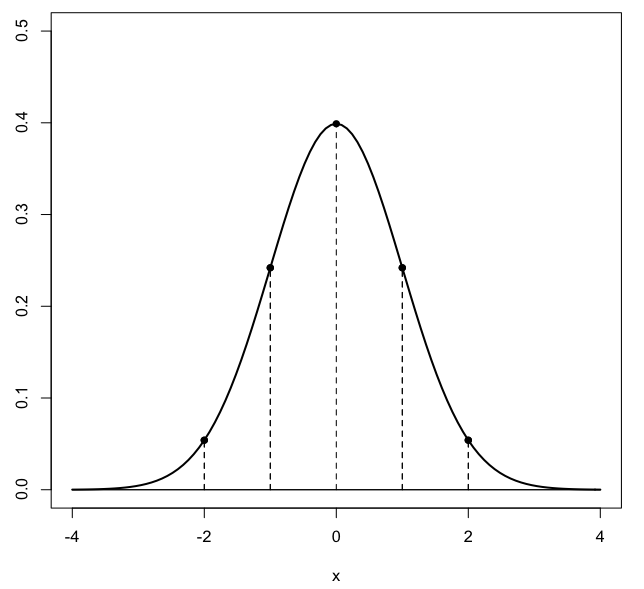
\includegraphics [scale=0.4] {gauss3.png} \end{center}
% \begin{bmatrix} a  &  b \\ c  &  d \end{bmatrix}
% \bigg |_

\begin{document}
\maketitle
\Large
%\noindent
This short write-up is a simple explanation of how and why PCA works.  To understand it you will first need to know something about eigenvalues and eigenvectors.  If you have a basic understanding of those already, then you should be fine.

It will also help if you have actually carried out PCA on some real data.  I'll show an example of that later.

We start with a data matrix $X$.  For example, suppose it's one where the properties of each amino acid are given:  mass, hydrophobicity and so on.  These are listed as numeric values $m$, $h$, $s$.

We organize the matrix with the values for each sample (Alanine through Tyrosine), organized as columns.

\[
\begin{matrix}
  &   & samples &  \\
  & A & => & Y \\
\text{mass} & m_1 &  & m_n \\
\text{hydrophobicity} & h_1 &  & h_n \\
\text{surface area} & s_1 &  & s_n
\end{matrix}
\]

With the samples organized into columns, values of similar type (e.g. mass) are found in the same row.

Now, subtract the mean for each row from each entry in that row.  This doesn't change the shape of the data but just shifts it in space so that it is centered around the origin (try it for a 2 by 2 matrix to see a simple example.  Of course, we're working in $n$-dimensional space but the idea is the same).

The covariance matrix of $X$, which we will call $A$, has entries formed by \emph{dotting} (multiplying) together rows of sample data.

If we think of both the rows and columns of $A$ as having general labels $x,y,z \cdots$, then the covariance of property $x$ and property $y$ would become the entry at row $x$, column $y$ ($a_{xy}$), and is calculated in the usual way as

\[ \frac{1}{n-1} \ \Sigma \ x_1 y_1 + x_2 y_2 + \cdots x_n y_n \]

The covariance matrix is a \emph{symmetric} matrix, since the covariance of $x$ with $y$ is equal to the covariance of $y$ with $x$, and the value at $a_{xy}$ is equal to the value at $a_{yx}$ in the matrix, $A$.

Because we've centered the data, we can get the same result, within the factor of $1/n-1$, by doing

\[ A = X X^T  \]

(Set up a simple example and try it to see).

If X had been organized with each sample in a different row and the values of a similar type in the same column, then we would do $X^T X$.  

The column oriented layout we're using here makes matrix multiplication look backward to me, but it is pretty standard for PCA and so I'm going to use it.  If you work an example and run into a problem, it may very well be due to that issue.

The goal of PCA is simply to find a particular matrix $P$ such that when we use $P$ to multiply $X$ and then find the covariance by
\[ PX (PX)^T \]
the matrix that we obtain is diagonalized.  That's the complete, sum total of what we're trying to do.

In other words, we want the end result $PX (PX)^T$ to look something like this
\[
\begin{bmatrix}
q & 0 & 0 & 0 \\
0 & r & 0 & 0 \\
0 & 0 & s & 0 \\
0 & 0 & 0 & t
\end{bmatrix}
\]

Think of $P$ as a transformation of the data to a new basis.  In this new basis, the resulting matrix $PX$ has all of its variance due to the variances of the individual properties (lying along the diagonal), with no covariance.

Let's push some letters around.  We have

\[ A = X X^T \]
and so $C$, the covariance matrix of $PX$, is
\[ C = (PX) (PX)^T  \]
using the identity $(PX)^T = X^TP^T$
\[ C = P X X^T P^T \]
and substituting $A$ back again for $X X^T$
\[ C = P A P^T \]

To restate what we're doing, we are looking for a matrix $P$ that will make $C = P A P^T = P X X^T P^T$ have the property of being diagonalized (with all the co-variance removed by concentrating it, if you will, in the variance).

$A$, the covariance matrix of $X$, is symmetric and real.  A fundamental result from linear algebra is that any symmetric real matrix has an eigen decomposition or factorization with real eigenvalues and orthogonal eigenvectors.  We are guaranteed to be able to find $D$ and $E$ with these properties, with
\[ A = E D E^T \]

where $E$ contains the eigenvectors of $A$ as columns, and these can easily be normalized to have unit length.  Since they are orthogonal and unit length (they are orthonormal)
\[ E E^T = I \]

Expanding our expression for $C$
\[ C = P A P^T = P E D E^T P^T \]

This looks like alphabet soup, but hang on, we're nearly there.  

Remember our goal:  to diagonalize $C$.  Notice that $D$ is a diagonal matrix.  How can we make $PE$ go away?

\emph{Brilliant idea}:  \emph{select} $P = E^T$.  Because of orthonormality
\[ PE = E^T E = I \]

So with this choice for $P$
\[ C = P A P^T = P E D E^T P^T = D \]

Remember how we obtained $E$ and $D$.  They come from the eigen decomposition of $A$ ($ = X X^T$), and $P = E^T$.

We're almost done.  What remains is to sort $E^T$ and $D$ (in corresponding order) from largest to smallest eigenvalue (actually R does this for you).  Then select (e.g.) the first two rows of $E^T$ as basis vectors in a matrix $M$.  Project $X$ onto that basis by just multiplying $X^* = M X$.

The variance for each principal component is the square root of the corresponding eigenvalue of $A = X X^T$.  Each pairwise covariance of the principal components is zero because they are orthogonal.

\subsection*{example}

Here is the setup, using Python.  

\begin{tt}
\begin{lstlisting}
import random
import numpy as np
import matplotlib.pyplot as plt
random.seed(153)
N = 50

X = [10*random.random() for i in range(N)]
Y = [random.random() for i in range(N)]
X = [x - np.mean(X) for x in X]
Y = [y - np.mean(Y) for y in Y]

M = np.matrix([X,Y])
plt.scatter(M[0],M[1],s=200,
    marker="o", color="0.8")
plt.axes().set_aspect('equal')

s = np.sqrt(3)/2.0
R = [[0.5,-s],[s,0.5]]
M = R * M
plt.scatter(M[0],M[1],s=100,color="salmon")
\end{lstlisting}
\end{tt}

What we've done so far generates 50 random points from the uniform distribution, stretched by a factor of 10 in the x-direction.  We plot the original points in light gray and then salmon colored points (rotated by 60 degrees counter-clockwise).  

The next part is the PCA, which will analyze the data to produce the correct matrix to rotate back.  The points that have been multiplied by the matrix are plotted in black.
\begin{center} 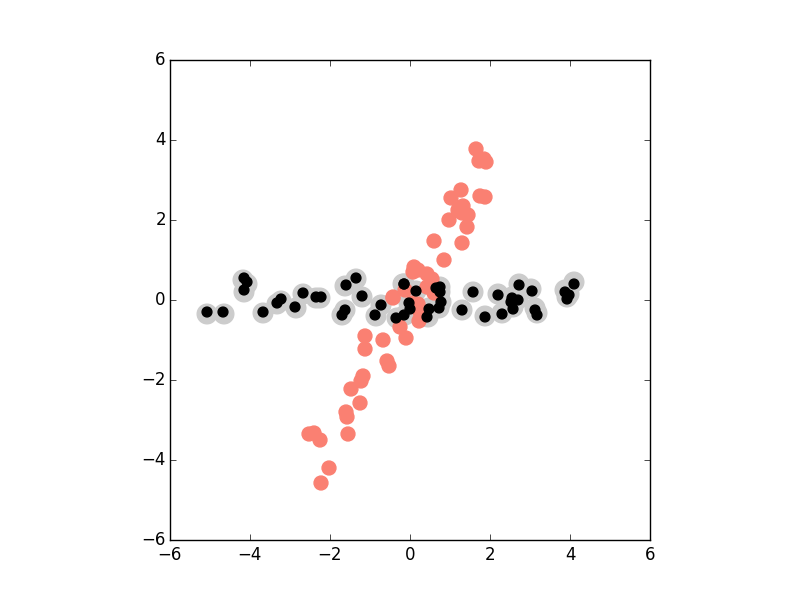
\includegraphics [scale=0.75] {pca_example.png} \end{center}

Here is the Python code for actually extracting the eigenvectors.

\begin{tt}
\begin{lstlisting}
A = M * M.transpose()
D,E = np.linalg.eig(A)
# evecs listed with evals in increasing order
# so switch the two columns
E = E[:,(1,0)]

M = E * M
# PCA may flip pos and negative, and did so here
M[0] = -M[0]
plt.scatter(M[0],M[1],s=50,color="black")
plt.savefig("example.png")
\end{lstlisting}
\end{tt}

The amount of the variance is the square root of the eigenvalue.  (The covariance of $x$ with itself is $(var(x))^2$.

\subsection*{SVD}

Singular Value Decomposition (SVD) is closely related to PCA.  We have

\[ A = X X^T = E D E^T \]

SVD takes the original $m \times n$ matrix $X$ and gives:

\[ X = U S V^T \]

with $U$ ($m \times m$) and $V^T$ ($n \times n$) both orthonormal and $S$ ($m \times n$) a diagonal matrix.  Notice:

\[ A = X^T X  \]
\[   = (U S V^T)^T (U S V^T) \]
\[   = V S U^T U S V^T \]

since $U$ and $V$ are orthonormal $U^T U = I$ so

\[ A = V S^2 V^T  \]

but for the eigen decomposition we had
\[ A = E D E^T \]
Thus
\[ E = V \]
\[ D = S^2 \]

SVD is said to be more stable numerically.

\end{document}  